\section{UX/UI}

Este módulo define la interfaz gráfica y las interacciones del usuario con el sistema (UI/UX), constituyendo el frontend de la aplicación. A través de esta capa, los usuarios pueden acceder a todas las funcionalidades del sistema de manera intuitiva y eficiente.

\subsection{Diseño/Navegabilidad}

\begin{figure}[H]
    \centering
    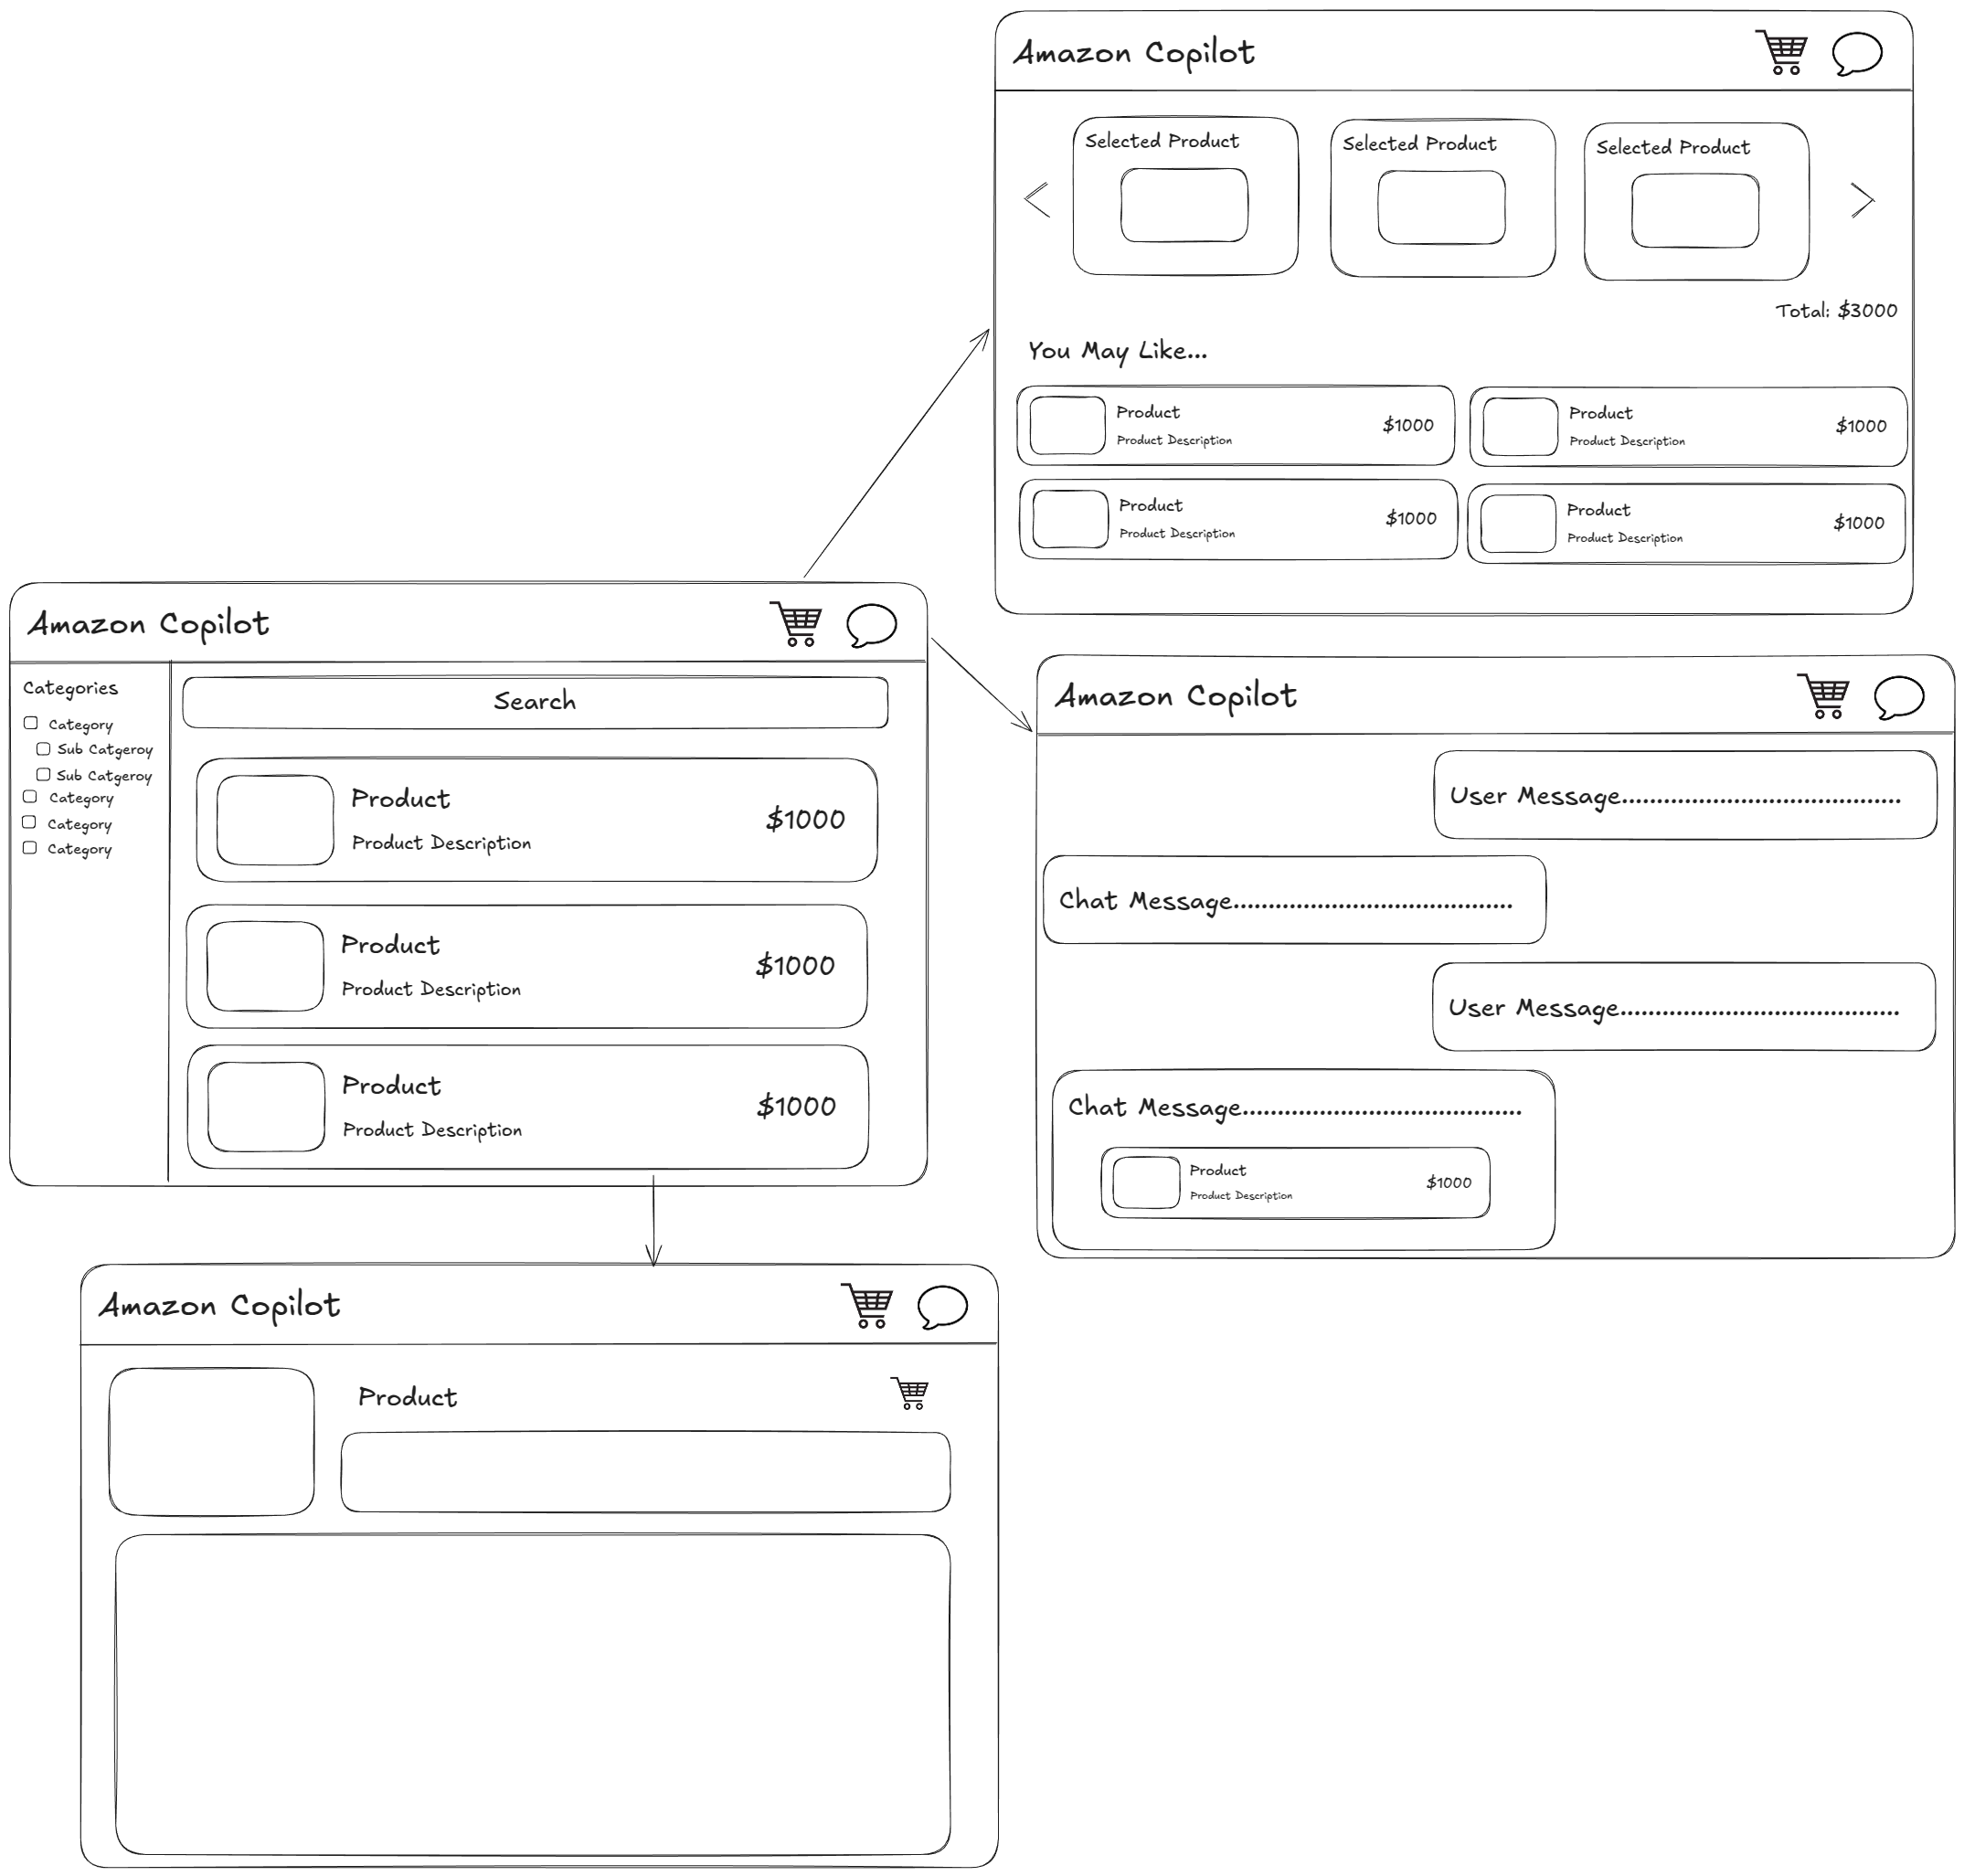
\includegraphics[width=0.8\textwidth]{ux.png}
    \caption{Diseño UX de la interfaz web.}
    \label{fig:ux_design}
\end{figure}

\noindent \textit{Nota: Este diagrama modela las interacciones del usuario con el sistema. El diseño final de la interfaz de usuario está pendiente de desarrollo.}

\vspace{0.75cm}

La interfaz permite al usuario: visualizar un listado inicial de productos con barra de búsqueda y filtros por categorías; realizar búsquedas que actualizan dinámicamente los resultados; acceder a detalles de productos específicos; gestionar un carrito de compras que muestra recomendaciones relacionadas; e interactuar con el asistente conversacional para búsquedas conversacionales, manteniendo el historial de la conversación.

\subsection{Filtros, Pagination}

El sistema implementará filtros avanzados que permitan a los usuarios refinar sus búsquedas por categoría, rango de precios, valoraciones y otros atributos relevantes. La paginación eficiente garantizará una experiencia fluida incluso con grandes volúmenes de resultados.

\subsection{Estado (Cart \& Conversation)}

La gestión del estado incluye el mantenimiento persistente del carrito de compras y el historial de conversaciones con el agente de IA. Esto permite una experiencia coherente y personalizada a lo largo de toda la sesión del usuario.
